\chapter{Architecture} \label{chap_method}

In this chapter we will present our suggested architecture for a hardware accelerated forward propagation of a Convolutional Neural Network used for recognizing handwritten digits. The architecuture will be presented in a top-down approach, starting with the topology and dataset of the network, followed by an overview of the software used, and finally, the hardware architecture of the accelerator. The source files for the VHDL and software code used in this project can for the time being be found at \cite{Halvorsen2015}

\begin{figure}[h!]
  \centering
      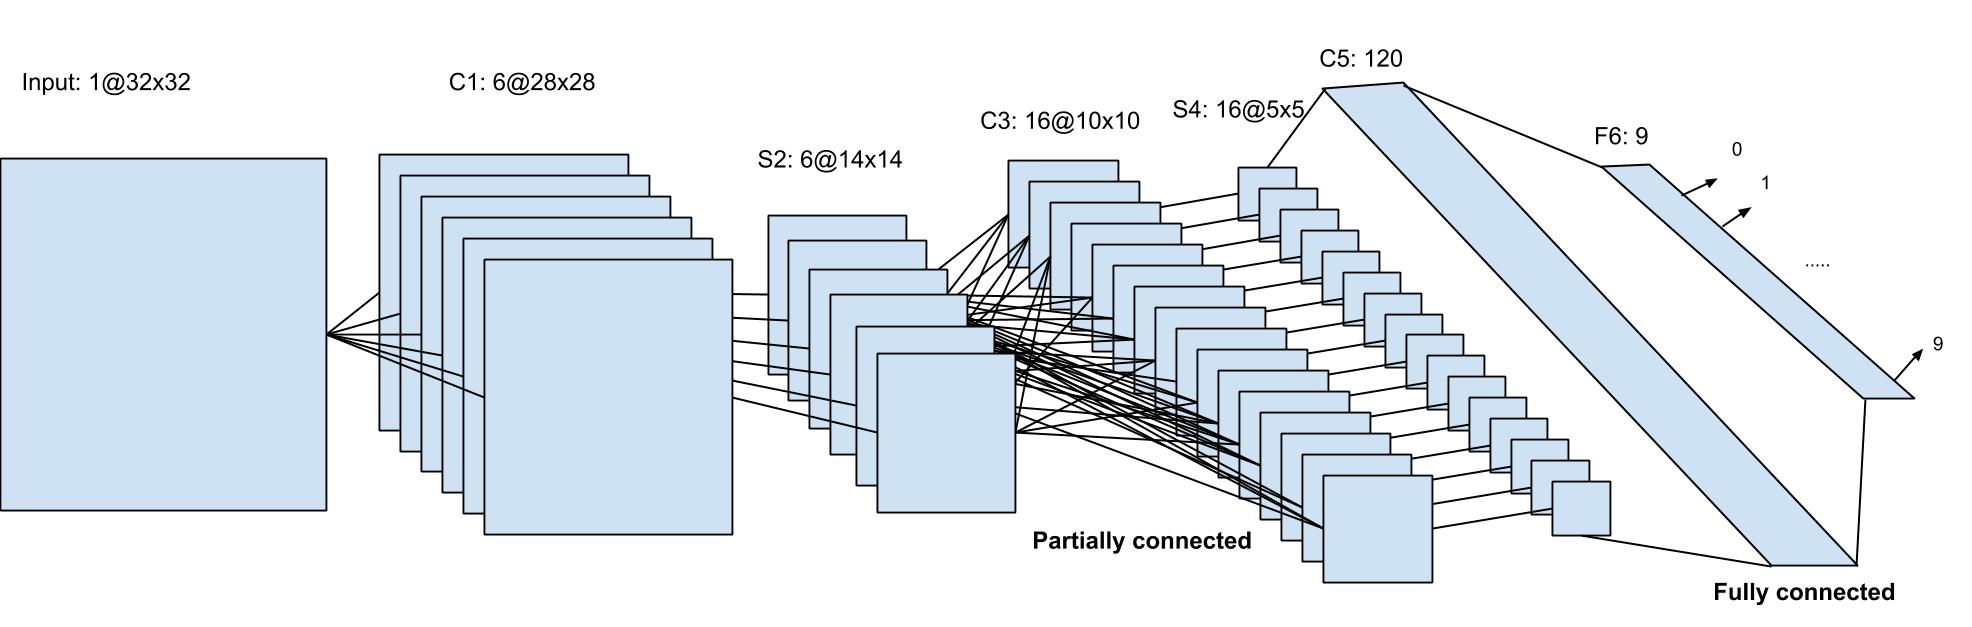
\includegraphics[width=1.2\textwidth, height=5cm]{Figures/Method/Network_topology}
    \caption{The topology of the implemented network.}
    \label{fig_network_topology}
\end{figure}

\section{Network Topology and Dataset}

We chose to implement a network with a smiliar topology as the LetNet-5 for digit recognition, as seen in Figure \ref{fig_network_topology}. It consist of six layers: 

\begin{itemize}
  \item \textbf{C1, convolution layer}. Takes in a single $ 32 \times 32 $ image of an digit. The image is convoluted using six different trained kernels, and outputs six respective $ 28 \times 28 $ feature maps. 
  \item \textbf{S2, subsampling/average-pooling layer.} Performs the subsample/average-pooling operation on each of the six $ 28 \times 28 $ feature maps from the previous layer, using a respective trained value for each map. The resulting output is six $ 14 \times 14 $ subsampled feature maps. 
  \item \textbf{C3, partially-connected convolution layer.} Takes in six $ 14 \times 14 $ feature maps which are partially connected to the sixteen $ 10 \times 10 $ output feature maps. These connections are shown in Table \ref{table_partial_connections}. The connections specifices which inputs are needed to compute a given output. E.g. in order to compute feature map 13, input 2, 4 and 5 are to be convoluted with the 13's kernel. The respective convoluted inputs are then combined into a single matrice, where a bias and activation function is applied to every element - which give the resulting output feature map. 
  \item \textbf{S4, subsampling/average-pooling layer.} Performs the subsample/average-pooling operation on each of the sixteen $ 10 \times 10 $ feature maps from the previous layer, using a respective trained value for each map. The resulting output is sixteen $ 5 \times 5 $ subsampled feature maps.
  \item \textbf{C5, fully connected convolution layer.} Takes in a sixteen $ 5 \times 5 $ feature maps which are fully connected to the 120 $ 1 \times 1 $ output feature maps. Since the size of the output feature maps are a single value, the feature maps are basically standard neurons. 
  \item \textbf{F6, output layer}. Takes in 120 neurons which are fully connected to the 10 output neurons. The output neuron with the highest value is the predicted value of the network. 
\end{itemize}


\begin{figure}[h!]
  \centering
      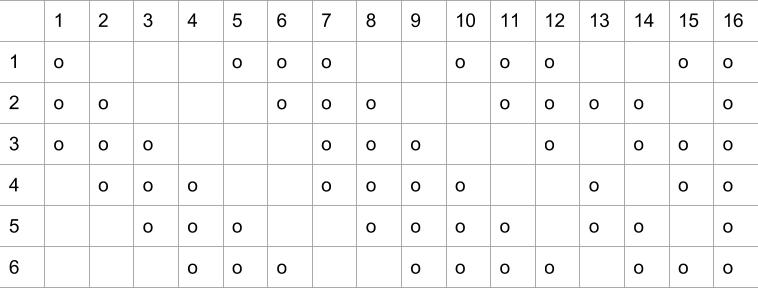
\includegraphics[width=1.0\textwidth]{Figures/Method/partial_connections}
    \caption{Table showing which of the six feature maps from S2 that are needed in order compute the feature maps of C3.}
    \label{table_partial_connections}
\end{figure}

There are three primary reasons for choosing this network. First, it is a relatively small network, which simplifies the implementation by reducing the chances of bugs and memory problems. Secondly, the kernel size of all the convolution layers are the same. This allowed for a less complex implementation, since we did not have to design our accelerator to support different kernel sizes, making it easier for the accelerator to support all the convolution layers. Thirdly, this network have been shown to work very well with the MNIST dataset, i.e. our own experiments gave an accuracy of 99.1\%. Since the aim of this project is exploring hardware acceleration, we did not wish to spend time finding a working topology for a given dataset. Using a topology that has been shown to give high accuracy allowed us to focus more on acceleration rather than topology theory.   

 As mentioned, we used the \textit{the MNIST dataset}, available at \cite{LeCun1998a}. It consists of 50 000 samples of handwritten digits ranging from 0-9, where 40 000 of the samples are used for
training and 10 000 samples are used to determine the accuracy of the network. 

\section{What to accelerate} \label{sec_what_to_accelerate}

In order to decide which part of the network that should be accelerated one has to determine the most computational expensive part of the network. In the literature (see Chapter \ref{chap_related_work}) there is a common consensus that the convolution layer is the most demanding layer, and \cite{Farabet2010} and \cite{Zhang2015} states explicitly that it amounts to about 90\% of the total processing. We have confirmed this number in our own experiments, through a simple mathematical analysis of the network and by profiling a software implementation of the network. 

\begin{table}
	\centering
    \begin{tabular}{| >{\centering\arraybackslash}m{0.8in} | >{\centering\arraybackslash}m{1.0in} | >{\centering\arraybackslash}m{1.0in} |}
    \hline
    Layer & Connections & Percentage  \\ \hline
    $ C1 $ & $ 122304 $ & $ 0.37 $ \\ \hline
    $ S2 $ & $ 5880  $ & $ 0.02 $ \\ \hline
    $ C3 $ & $ 151600 $ & $ 0.46 $  \\ \hline
    $ S4 $ & $ 2000 $ & $ 0.006 $ \\ \hline
    $ C5 $ & $ 48120 $ & $ 0.14 $  \\ \hline
    $ F6 $ & $ 120 $ & $ 0.004 $ \\ \hline
    $ Total $ & $ 331104 $ & $ 1.0 $  \\ \hline
        \end{tabular}
    \caption{An overview of the number of connections in the network layers.}
   	\label{tab_nofOps}
\end{table}

Table \ref{tab_nofOps} shows the number of connections for each layer in the network. Each connection corresponds to a multiply-and-accumulate (MAC) operation, e.g. 122304 MAC operations are required to compute C1. Since the number of activation functions to be computed is strongly correlated to the number of connections, we refrained from including them in the analysis. 
We see that 97\% of the computations in our network is performed in the convolution layers, giving a clear indication of what layers should be accelerated.


We also decided to accelerate the subsampling/pooling layers, even though only 0.8\% of computations are done there. The reason for this that we were able to make a design where the subsampling/pooling could be done virtually in parallel with the convolution, at a minimal cost to hardware resources (see Section \ref{sec_average_pooler}. We deemed the small cost worth the 0.8\% potential performance boost. But more importantly, it makes our architecture eaiser to extend to compute several layers in a row, without going back to software, which would greatly reduce off-chip traffic and performance (see Chapter \ref{chap_future_work}).

%%%%%%%%%%%%%%%%%%%%%%%%%%%%%%%%%%%%%%%%%%%%%%%%%%%%
% Software
%%%%%%%%%%%%%%%%%%%%%%%%%%%%%%%%%%%%%%%%%%%%%%%%%%%%

\section{Software Architecture}

This section gives an overview of software architecture used to compute the network and to control the accelerator.

\subsection{Network Software}

We have made extensive use of Taiga Nomi's C++ framework for neural networks, available at \cite{Nomi2015}, in our project. The framework was used in order to train the parameters of our network, for measuring the efficency of a pure software implementation, and as a basis for the implementation that uses the hardware accelerator. The framework treats each layer in the network as a seperate software module, which makes it easy to swap diffrent implementations of a layer. This simplified the process of integrating the hardware accelerator into the network, since we could simply exchange the original modules with our own.

Figure \ref{fig_software_architecture} A shows a simplified version of the architecture of the pure software implementation of our network. Each layer contains a set of pretrained weights which are loaded before the network starts processing the images. When an image is inputted to the first layer, it performs the calculations described in Chapter \ref{chap_background} in software, and propegates the result to the next layer. 

Figure \ref{fig_software_architecture} B shows how the original software was changed in order to make use of the accelerator. As mentioned, we decided to accelerate the convolutional layer and the subsample/average-pooling layer, thus we wrote a new software module that would handle both operations. But instead of computing the operations in software, the new module transfers the input data and the weight to the hardware accelerator and extracts the result from the computations. 

While our architecture supports accelerations of C5, we refrained from using it in its current form. The reason being that currently the accelerator is only able to compute one feature map at a time. Each computation comes with a certain amount of overhead, i.e. transfering data to/from the accelerator and configuring it. Thus for C5, which takes in 120 $ 5 \times 5 $ matices, we figured that input was so numerous and so small that it would cause too much overhead in order to be efficient. In Chapter \ref{chap_results} we show data that confirms this claim.


\begin{figure}[h!]
  \centering
      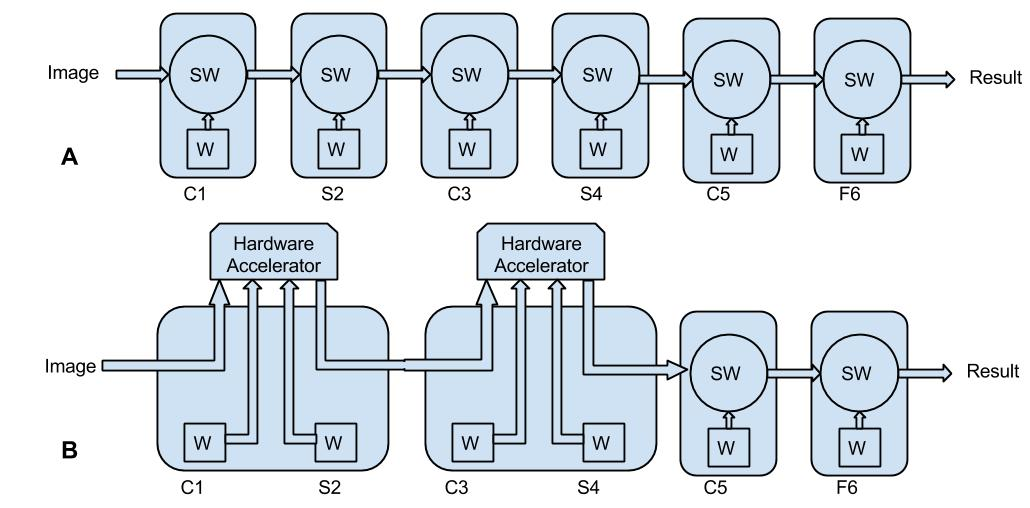
\includegraphics[width=1.0\textwidth]{Figures/Method/SoftwareArchitecture}
    \caption{A simplified overview of the software architecture with and without hardware acceleration.}
    \label{fig_software_architecture}
\end{figure}

\subsection{Hardware driver} \label{sec_hardware_driver}

A driver for the accelerator was written in order to create a simple and easy to use interface to the hardware. As mentioned, in its current form the accelerator is able to compute on feature map at a time, thus the input to the driver is all the data required to compute said feature map. That is, a set of images, their respective kernels and bias, the average pooling constant and its respective bias. The driver then feeds this data to the accelerator, and returns the computed feature map. Due to the architecture of the accelerator the input has to be transfered in a certain order. The biases and average pooling constant first, the weights second and the image last. Figure \ref{fig_fifo_content} shows in what order the data should be in the accelerator FIFO buffer.


\begin{figure}[h!]
  \centering
      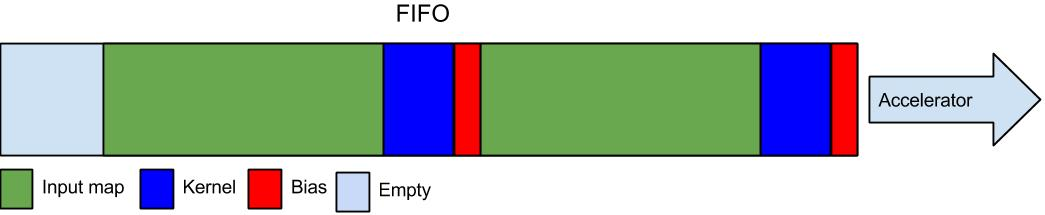
\includegraphics[width=1.0\textwidth]{Figures/Method/FIFO_content}
    \caption{Shows how the data must be sequentially ordered in the input FIFO. In this example the output feature map is computed using two input maps.}
    \label{fig_fifo_content}
\end{figure}

For data transfer the driver uses a \textit{direct memory access controller} (DMA) IP from Xilinx. This is where most of work on the driver had to be done, since the DMA interface is much more complex compared to the accelerator interface. The DMA is configured to transfer the weights and image(s) to the accelerator's input buffer, and extract the data from the output buffer. Since the output buffer is a FIFO, the DMA is able to extract each output value as they are produced, instead of waiting for the accelerator to finish and then transfer all the output data. Figure \ref{fig_fifo_content} shows how the data has to be structured when transfered to the accelerator's input buffer.

The processor can make use of the DMA by providing it with a set of \textit{buffer descriptors} (BD), also called a BD ring. Each descriptor provides the DMA with the neccessary information to perform a memory transfer: a source address and/or a destination address (depends on type of channel), and the length of the packet to transfer. One also need to set a \textit{start of file}(SOF) and \textit{end of file} (EOF) control bit for the first and last BD in the ring, respectively. 

Our DMA has two channels, a transmit (Tx) and receive (Rx) channel. For the Tx channel the destination of the data is set to the address of the component connected to the DMA's Tx bus. Which in our case is the buffer which feeds the accelerator. Similary, the Rx channel's source address is set to the component connected to the Rx bus, i.e. the FIFO buffer containing the output of the accelerator.

E.g. if a feature map requires two sets of input maps, weight and bias, then Figure \ref{fig_bdring} shows a simplified version of the Tx BD ring. Since the BDs are processed sequentially, the data will be transfered in the correct order, as in Figure \ref{fig_fifo_content}.

\begin{figure}[h!]
  \centering
      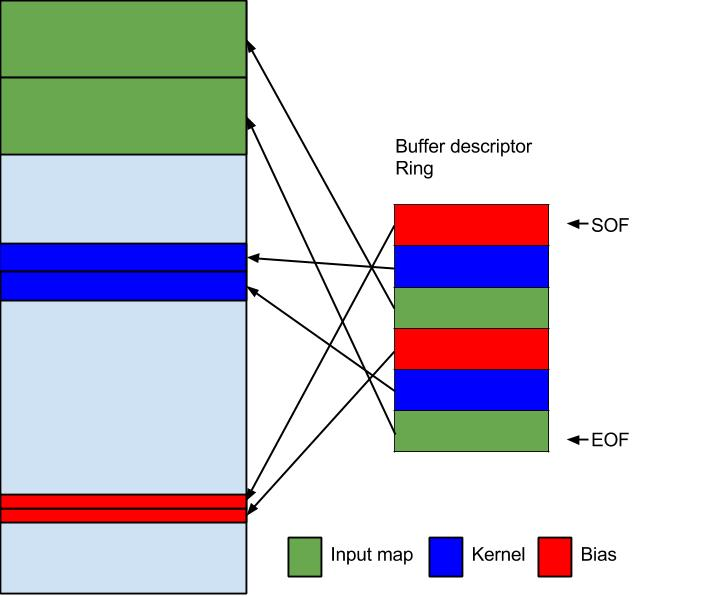
\includegraphics[width=0.7\textwidth]{Figures/Method/BdRing}
    \caption{Simplified version of the Tx BD ring. First BD points to the location of the bias, second to the weights, and the third to the image, etc.}
    \label{fig_bdring}
\end{figure}


Xilinx provides a software driver for the DMA that manages the BD rings and initializes DMA transfers. A subset of the driver interface is listed below, showing the functions we used to control the DMA. For a more detailed explaination of the interface, please refer to the documentation in the driver source code, available at \cite{DMA_DRIVER_SOURCE}


\begin{lstlisting}[caption={XAxiDma driver interface},label=dma_interface]

/* Retrievies the config structure required to initialize the DMA. */
Config* XAxiDma_LookupConfig(u32 XAxiDma_id);

/* Initializes the DMA */
int XAxiDma_CfgInitialize(XAxiDma *dma, XAxiDma_Config *config);

/* Returns a pointer to the BD ring for the Rx channel */
XAxiDma_BdRing* XAxiDma_GetRxRing(XAxiDma *XAxiDmaInstPtr);

/* Returns a pointer to the BD ring for the Tx channel */
XAxiDma_BdRing* XAxiDma_GetTxRing(XAxiDma *XAxiDmaInstPtr);

/* Returns the maximum number of BDs given the available memory size */
int XAxiDma_BdRingCntCalc(u32 bd_size, u32 size_of_available_memory);

/* Allocatetes memory for storing the BD ring */
int XAxiDma_BdRingCreate(XAxiDma_BdRing *RxRingPtr, u32 BaseAddr, u32 BdSize, u32 BdCount);

/* Allocated a number of BDs from the BD ring, which can be configured at submitted for hardware processing */
int XAxiDma_BdRingAllc(XAxiDma_BdRing *BdRingPtr, u32 BdCount, XAxiDma_Bd *FirstFreeBdInRing);

/* Sets of address the packet the BD should transfer. */
int AxiDma_BdSetBufAddr(XAxiDma_Bd *BdPtr, u32 addr);

/* Sets the length of the packet the BD should transfer */
int AxiDmaBdSetLength(XAxiDma_Bd *BdPtr, u32 length);

/* Set control signals for BD. E.g. SOF and EOF. */
XAxiDma_BdSetCtrl(XAxiDma_Bd *BdPtr, u32 CtrlMask);

/* Starts the channel. I.e. the DMA will start processing BDs as soon as they are submitted to hardware */
int XAxiDma_BdRingStart(XAxiDma_BdRing *BdRingPtr);

/* Submits the BD ring to hardware. Can not be accessed again before hardware is done processing. */
int XAxiDma_BdRingToHw(XAxiDma_Bdring *BdRingPtr, u32 BdCount, XAxiDma_Bd *FirstBd);

/* Extracts BDs from hardware after they are processed. Returns maximally BdCount BDs from hardware, but perhaps less */
int  XAxiDma_BdRingFromHw(XAxiDma_BdRing *BdRingPtr, u32 BdCount, XAxiDma *FirstBdRetrived);

/* Frees BdCount BDs after they have been processed by hardware. Must be done before the can resused for other transfers */
XAxiDma_BdRingFree(XAxiDma_BdRing *BdRingPtr, u32 BdCount, XAxiDma_Bd *FirstBdToFree);
\end{lstlisting}

Below we will show in simplified C code how we have used the above interface to configure and run, and transfer data to and from the accelerator. 

The first thing that has to be done is to initialize the DMA driver, allocate memory for the Tx and Rx BD rings, and start the channels.

\begin{lstlisting}

  void initializeDMA() {
    XAxiDma Dma;
    XAxiDma_Config *Config = XAxiDma_LookupConfig(DmaId);
    XAxiDma_CfgInitialize(&Dma, Config);

    SetupTx(&Dma);
    SetupRx(&Dma);
  }

  void SetupTx(XAxiDma *Dma) {
    XAxiDma_BdRingPtr *TxRing = XAxiDma_GetTxRing(Dma);
    int BdCount = XAxiDma_BdringCntCalc(MINIMUM_ALIGNMENT, TxBdMemorySpaceHigh-TxBdMemorySpaceBase);
    XAxiDma_BdRingCreate(TxRing, TxBdMemorySpaceBase, MINIMUM_ALIGNMENT, BdCount);
    XaxiDma_BdRingStart(TxRing);
  }

  void SetupRx(XAxiDma *Dma) {
    /* Virtually the same as SetupTx */
  }
  
\end{lstlisting}

This should only be neccessary to do once, as long as one does not need more BDs than what is currently allocated. Afterwards one can transfer data to the accelerator, run the accelerator and retrieve the output the following way: 

\begin{lstlisting}

  void computeOutputMap(XAxiDma *Dma) {

    SetupTransferToAccelerator(Dma);
    SetupTransferFromAccelerator(Dma);
    WaitForTx(Dma);
    RunAccelerator();
    WaitForRx(Dma);
    
  }

  void SetupTransferToAccelerator(XAxiDma *Dma) {

    XAxiDma_Bd *Bdptr;
    int BdCount = NumberOfInputMaps*3; /* Multiply with three, because each input map needs to transfer three packets: bias, weights and image. */
    XaxiDma_BdRing *TxRing = XAxiDma_GetTxRing(Dma);
    XAxiDma_BdRingAlloc(TxRing, BdCount, &BdPtr); 

    int index = 0;
    for each input map {
      for bias, weight and input map {
        XAxiDma_BdSetBufAddr(BdPtr[index], PacketAddr);
        XAxiDma_BdSetLength(BdPtr[index], LengthOfPacket);
        index++;
      }
      
    }
    XAxiDma_BdSetCtrl(BdPtr[0], SOF); /* First Bd in ring */
    XAxiDma_BdSetCtrl(BdPtr[BdCount-1], EOF); /* Last Bd in ring */

    XAxiDma_BringToHw(TxRing, BdCount, BdPtr[0]);
    
  }

 void  SetupTransferFromAccelerator(XAxiDma *Dma) {
    int BdCount = 1; /* Only need to retrieve one output map */
    XAxiDma_bd *BdPtr;
    XAxiDma_BdRing *RxRing = XaxiDma_GetRxRing(Dma);
    XAxiDma_BdRingAlloc(RxRing, BdCount, &BdPtr);
    XAxiDma_BdSetBufAddr(BdPtr, PacketAddr); /* specifies where the output map should be stored */
    XaxiDma_BdSetLength(BdPtr, PacketLength);
    XaxiDma_BdRingToHw(RxRing, BdCount, BdPtr);
 }

 void WaitForTx(XAxiDma *Dma) {
   XAxiDma_Bd *BdPtr;
   XaxiDma_BdRing *TxPtr = XAxiDma_GetTxRing(Dma);

   /* Get processed Bds from hardware */
   int ProcessedBdCount = 0;
   while (ProcessedBdCount < TotalBdCount) {
     ProcessedBdCount += XAxiDma_BdRingFromHw(TxPtr, TotalBdCount, BdPtr);
   }

   /* Free all Bds when transfer is complete */
   XAxiDma_BdRingFree(TxPtr, ProcessedBdCount, BdPtr);
 }

 void WaitForRx(XaxiDma *Dma) {
   /* Virtually the same as WaitForTx */
 }
\end{lstlisting}

The interface to the accelerator is designed to be as easy to use as possible, and requires little configurations. One simply needs to specify the layer that is going to be processed and the number of input maps that is needed to compute the output map. In addition, it is vitual that the input data is in the accelerators input buffer before it is started. With this is mind, the accelerator can be used in the following way:

\begin{lstlisting}
  void RunAccelerator() {
  	Xil_Out32(AcceleratorAddr+4, layer); //Set current layer
	Xil_Out32(AcceleratorAddr+8, nof_input_mapsx); //Set the number of input maps
	Xil_Out32(AcceleratorAddr, 0); //Start processing
  }
\end{lstlisting}

Where Xil\_Out32(u32 addr, u32 value) writes \textit{value} to the memory location of \textit{addr} in the PL. 



%% \begin{figure}[h!]
%%   \centering
%%       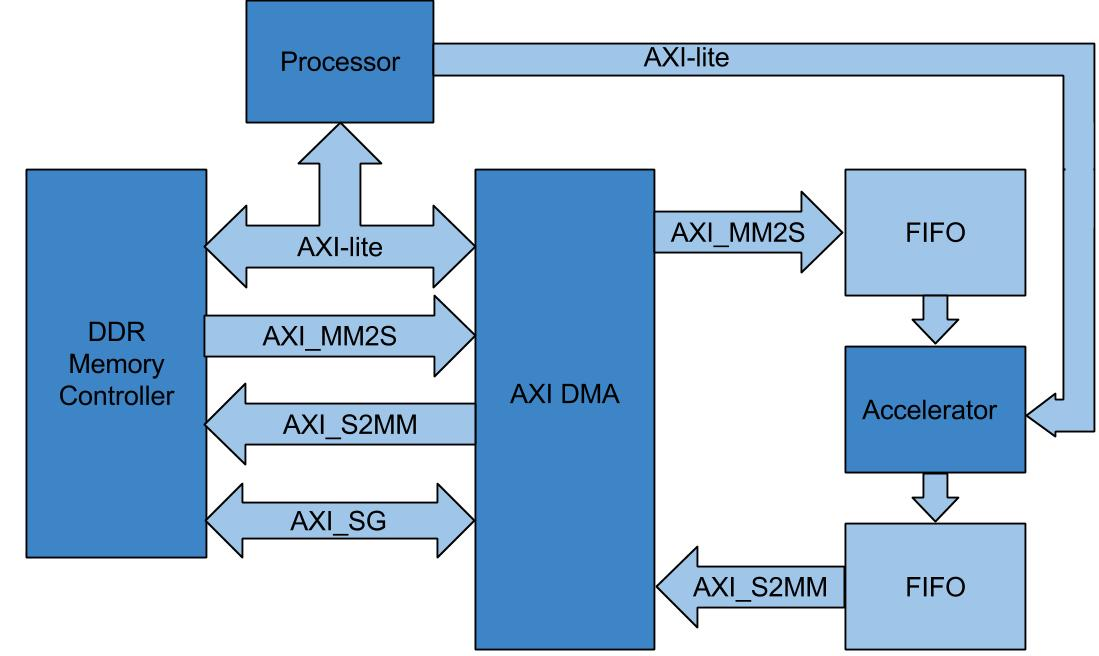
\includegraphics[width=1.0\textwidth]{Figures/Method/DriverAcceleratorInteraction}
%%     \caption{The interaction between the driver, DMA and accelerator.}
%%     \label{fig_driver_acc_interact}
%% \end{figure}
 


\begin{figure}[h!]
  \centering
      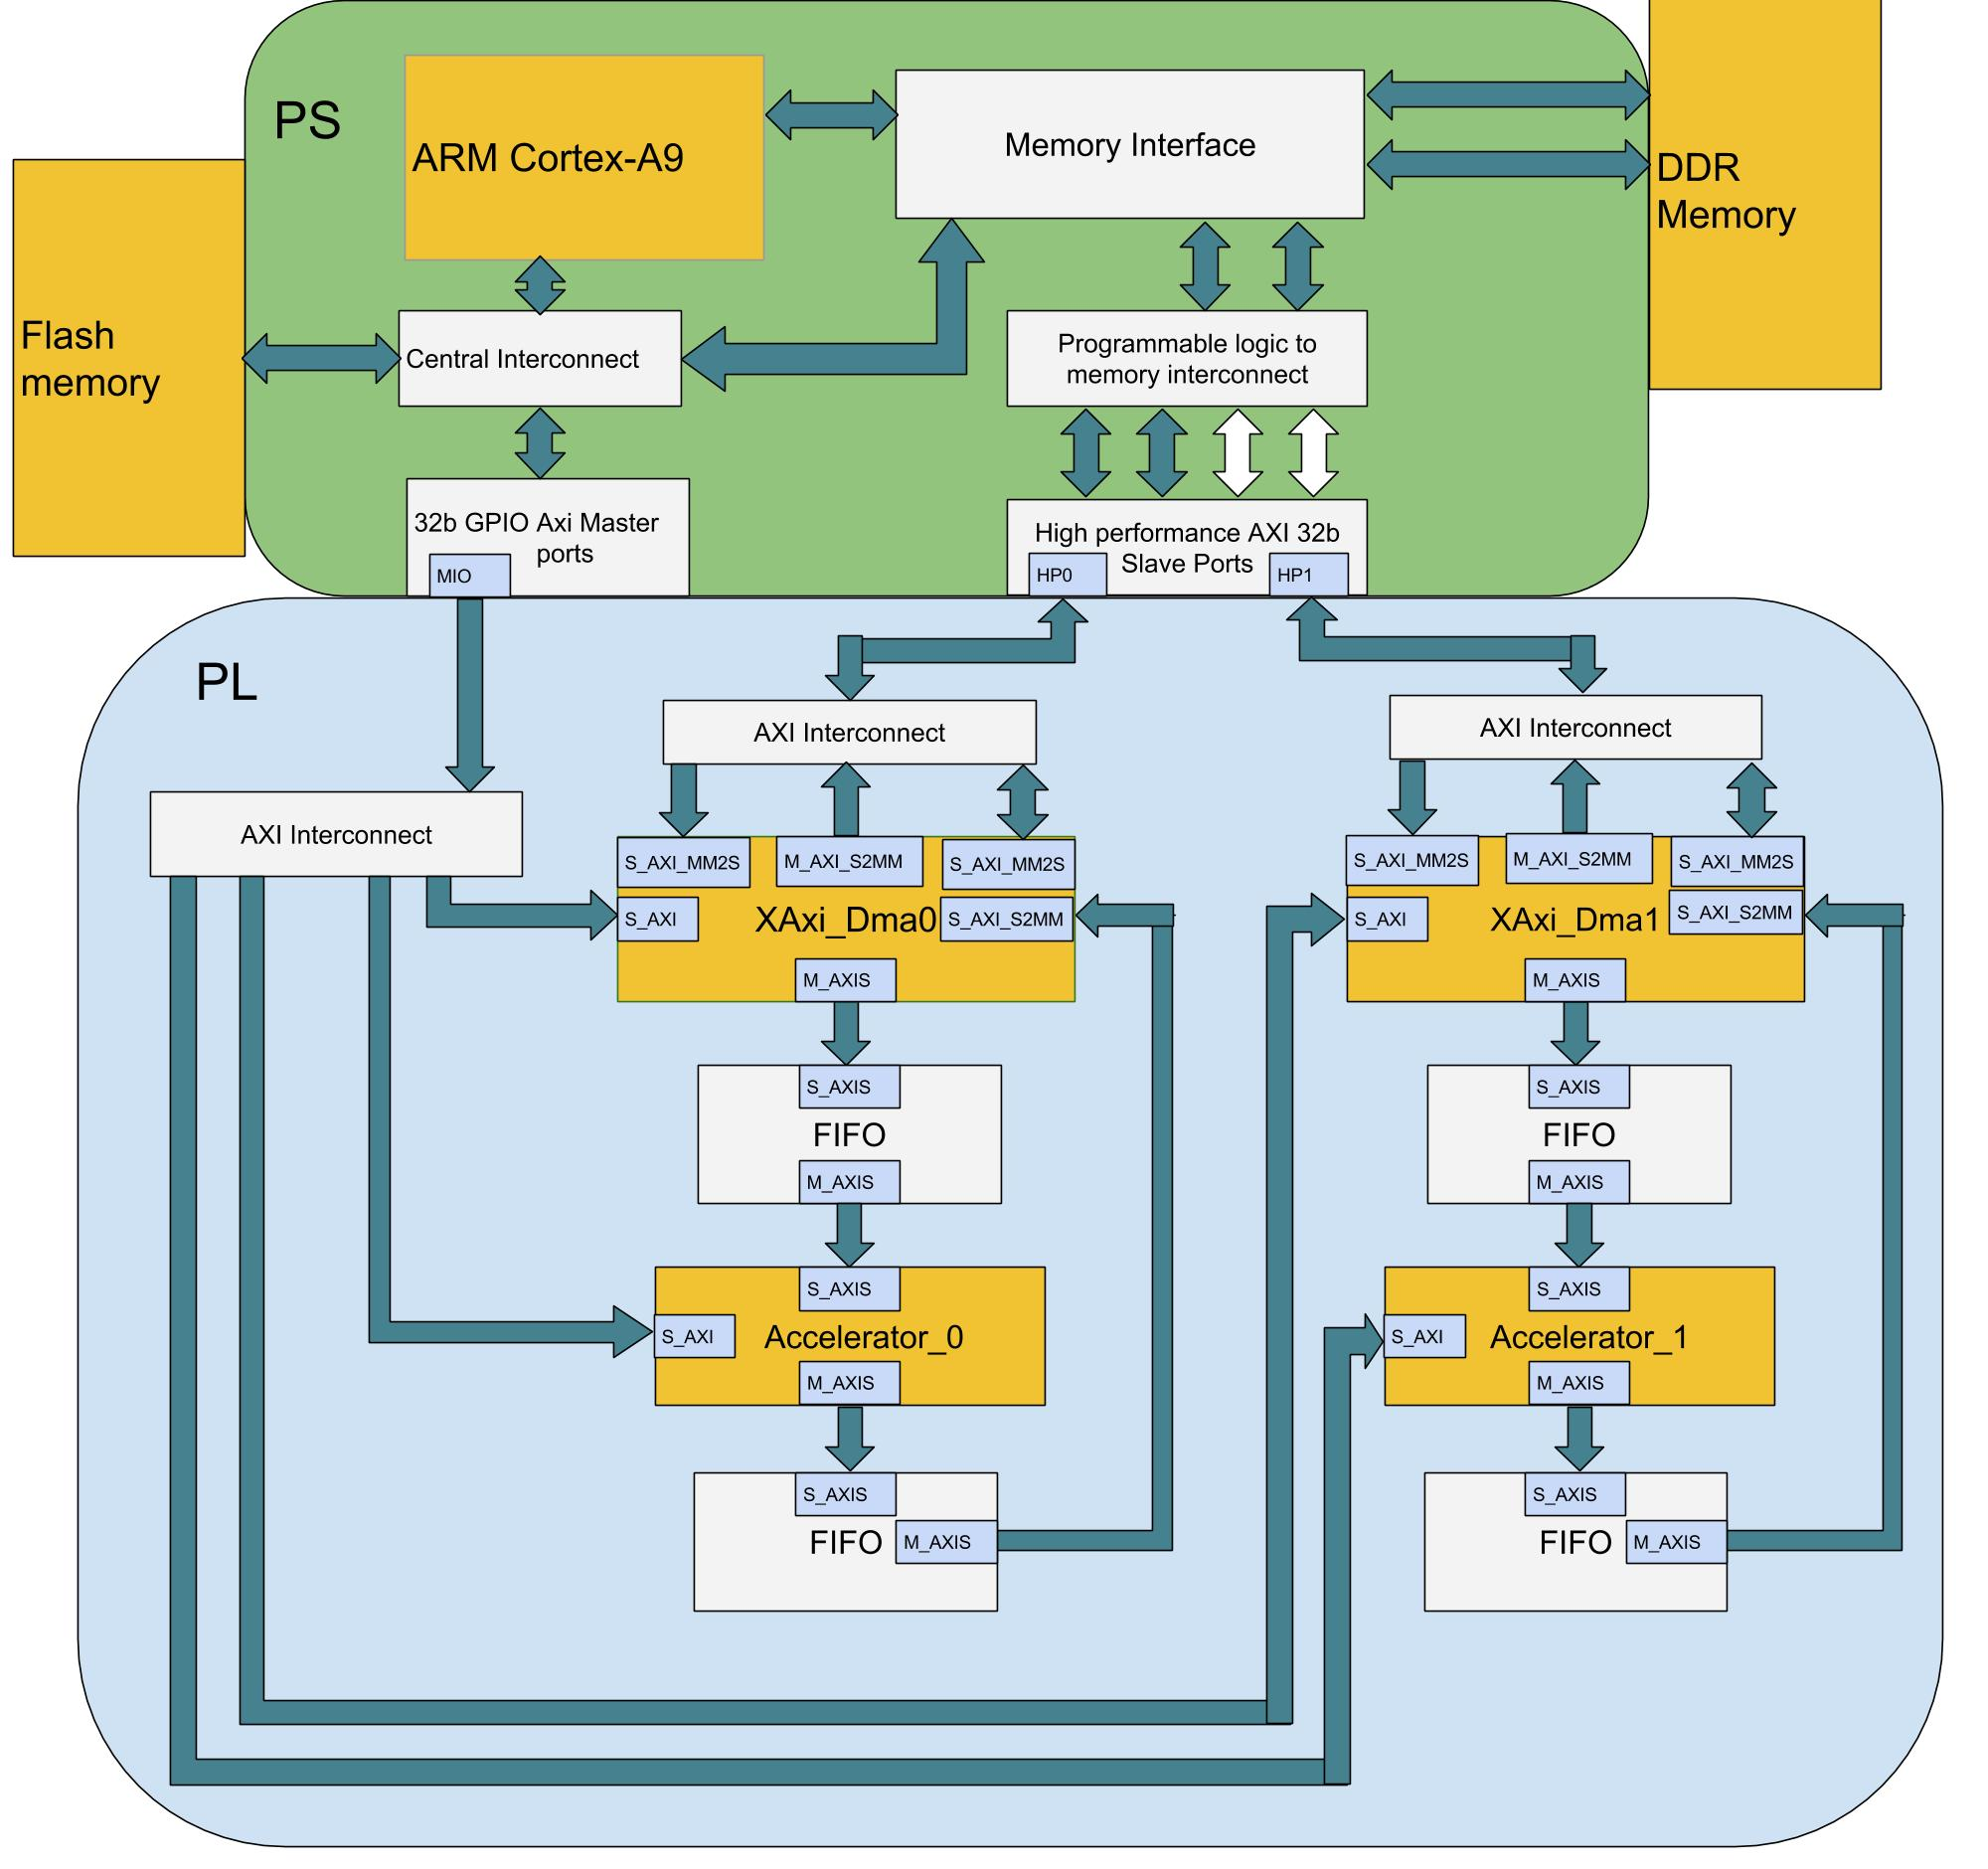
\includegraphics[width=1.0\textwidth]{Figures/Method/system_architecture}
    \caption{The system architecture.}
    \label{fig_system_architecture}
\end{figure}

\section{Hardware Architecture}

In this section we will describe the hardware architecture of the system as a whole, and more specifically, our accelerator. Do note that the descriptions and the figures are simplified to some extent. This simplication is done with the intent avoiding complex description and explainations. We will rather focus on conveying the important ideas behind the design, instead of describing every tiny detail of the architecture. 

\subsection{Overview of Hardware Achitecture}

Figure \ref{fig_system_architecture} shows the block diagram of our system architecture. In this design we have to accelerators running in parallel, with their own respective DMA which is used to feed them data. The DMA's are connected to two of the four available \textit{high performance AXI} ports, which are optimized for high bandwidth access from PL to external memory. The DMA has three bus interfaces that uses the HP ports:

\begin{itemize}
\item The AXI slave port \textit{Memory-Mapped to Streaming} (S\_AXI\_MM2S) is used to transfer data from memory to the DMA. All the data transfered by the DMA's Tx channel is transfered to this port. The data can than be rerouted to any arbitary hardware module, as long as they implement a S\_AXIS bus port which is connected to the DMA's M\_AXI\_MM2S port. 
\item The AXI master port \textit{Stream to Memory-Mapped} (M\_AXI\_S2MM) is used to transfer data from the DMA to external memory. The DMA receives data from the \textit{S\_AXI\_S2MM} which it rerouted to the M\_AXI\_S2MM if the Rx channel is active.
\item The \textit{Scatter-Gather} (SG) is used to transfer BDs between software and hardware. I.e. when software is done configuring the BDs and submit them to DMA control, the DMA transfers the BDs from memory to itself, and starts processing them. When the DMA is done processing the BDs are returned to memory through the same port. 
\end{itemize}

In order to configure and run the DMA, the processor is connected to it with a S\_AXI bus. This is used to tell the DMA where in memory it can find the BD ring, when BDs are ready for processing etc.

The accelerators are connected to two FIFOs, one for input and the other for output. The DMAs fill the input FIFO with data which the accelerator consumes, and extracts the accelerator's output data from the output FIFO. The processor can configure the accelerator directly by writing to it via the S\_AXI port.

The flash memory is used to store the trained parameters of the neural network, and the input images and their respective labels. When the application starts up, this data is parsed by the processor and then stored in the external memory, so it can be accessed by the DMA later on.  



\begin{figure}[h!]
  \centering
      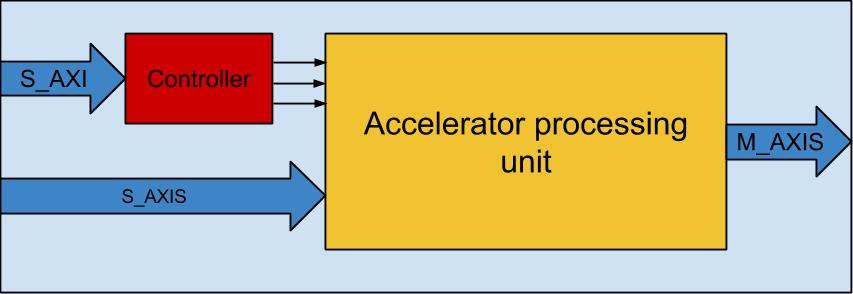
\includegraphics[width=0.9\textwidth]{Figures/Method/accelerator_interface}
    \caption{The interface of the accelerator.}
    \label{fig_accelerator_interface}
\end{figure}


\subsection{Accelerator Interface}

Figure \ref{fig_accelerator_interface} shows the block diagram for the interface of the accelerator. The S\_AXI bus, which the processor uses to configure the accelerator, is connected to a controller. The input maps, weights and biases are streamed into the processing unit via the S\_AXIS bus, and the resulting output map is streamed out via the M\_AXIS bus.

The controller is a state machine which controls the processing unit. It has three states: idle, loading weights and processing, as seen in Figure \ref{fig_accelerator_state_machine}. 

\begin{figure}[h!]
  \centering
      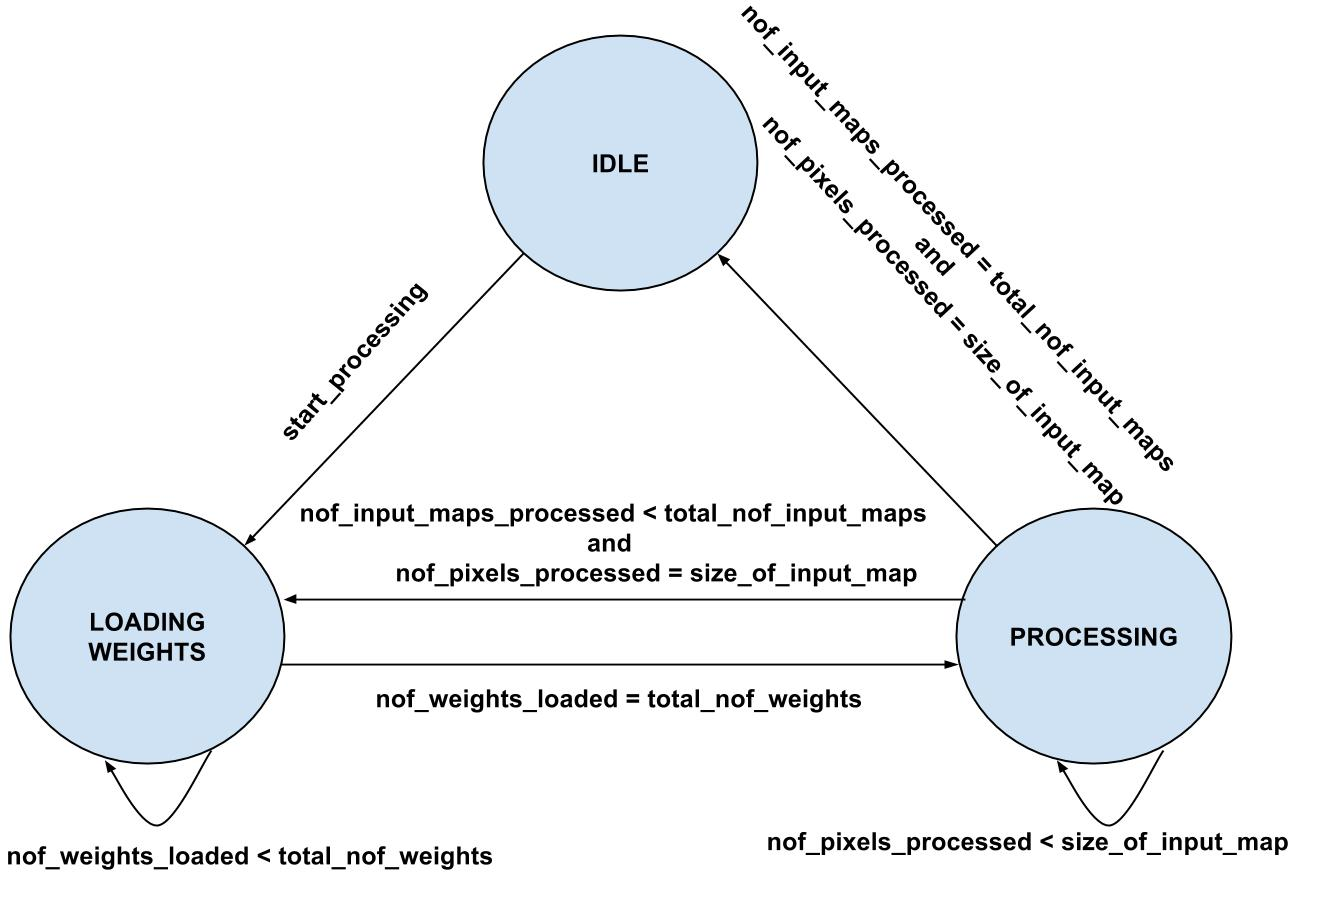
\includegraphics[width=0.9\textwidth]{Figures/Method/accelerator_state_machine}
    \caption{The three states of the accelerator's controller.}
    \label{fig_accelerator_state_machine}
\end{figure}

  
\subsection{The Accelerator's Processing Unit}

As previously stated, the accelerator takes \textit{n} images as input, $ I_1, I_2, \dots, I_n $, n respective kernels $ K_1, K_2, \dots, K_n $, two biases and an average pooling cofficient, and outputs a single processed image $ O $. Using the input images, the kernel and the bias, it performs the operations of the convolution and subsampling/average-pooling layer for a single feature map. Thus the output $ O $ is a subsampled/pooled feature map that has been produced by convoluting the images $ I_1, I_2, \dots, I_n $ with the kernels $ K_1, \dots, K_n $. 

The accelerator can thus compute the whole convolution and subsample/pooling layer by doing the above computations for all the output feature maps in the layer. One can exploit inter-parallelism by making several instances of the accelerator run in parallel. One can also exploit intra-parallelism, but then one need to connect the different accelerator instances so they can add up the results from the convolutions without using the intermediate convolution buffer, as described in \cite{Chakradhar2010}. Unfortunately, within the given timeframe we were unable to get a system working that exploited inter- and intra parallelism. But the architecture is designed to be easily extendable to support this, given more development time. 


The accelerators consists of five major components (Figure \ref{fig_imagezor_architecture}):

\begin{itemize}
	\item \textbf{The convoluter}. Performs the convolution operation on the input.
	\item \textbf{The intermediate convolution buffer}. Since the resulting feature map is the sum of the convolutions of all the input images (with the exception of the first layer), this buffer is needed to store the intermediate results from the previous convolution, so that it can be accumulated with the current convolution. In the first layer of the network there is only one input image (i.e. $ n = 1 $), thus no summation is needed.
	\item \textbf{Tanh}. Performs the non-linear hyperbloc tangent function  on the feature maps.
	\item \textbf{Subsample/average-pooler}. Performs the subsample/average-pool operation on the feature map. 
\end{itemize}

\begin{figure}[h!]
	\centering
    	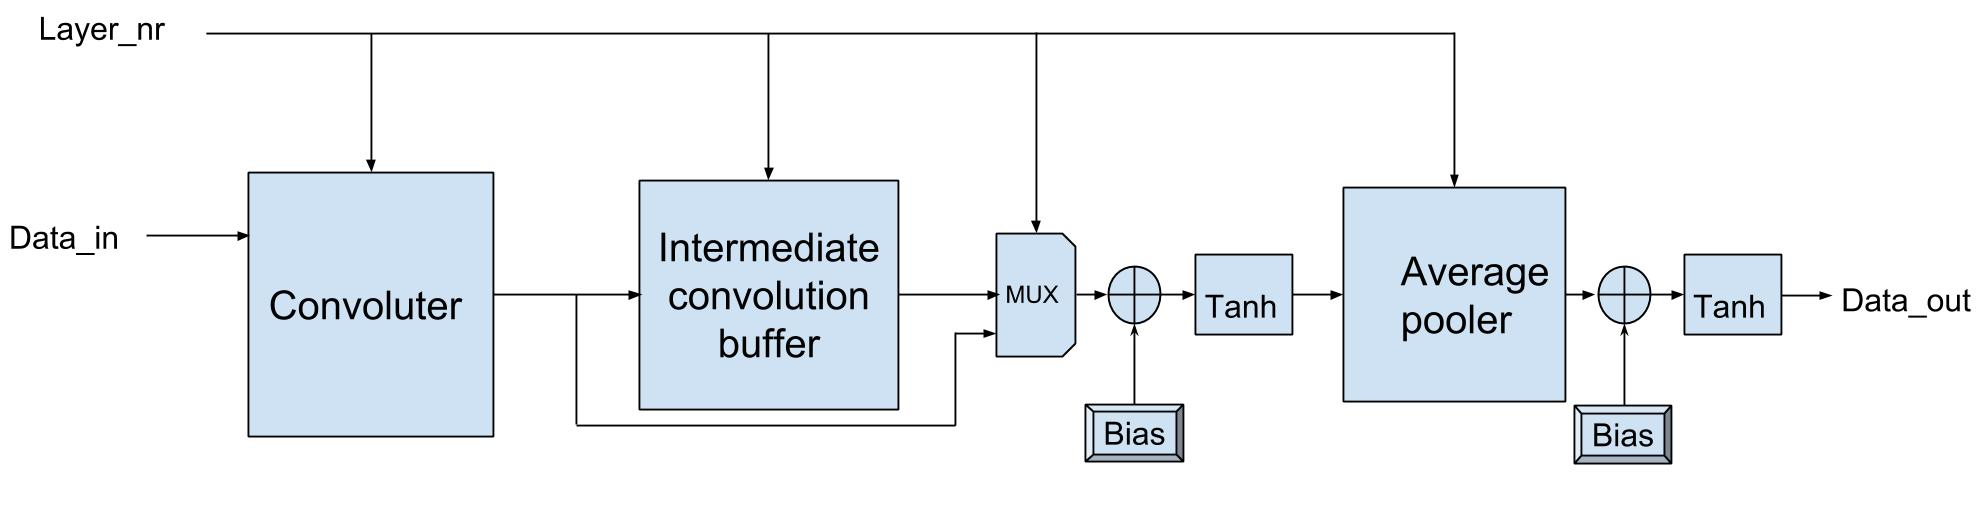
\includegraphics[width=1.0\textwidth]{Figures/Method/conv_layer_arch}
  	\caption{The architecture of Imagezor.}
  	\label{fig_imagezor_architecture}
\end{figure}

The \textit{layer\_nr} signal is used to specify whether it is C1/S2 or C3/S4 that is being computed. The input image in the first layer is bigger than the images in the second ($ 32 \times 32 $ vs $ 14 \times 14 $), which the convoluter and the average pooler need to  (see Section \ref{sec_convoluter} and \ref{sec_average_pooler}). In addition in the second layer the intermediate convolution buffer needs to be activated so it accumulate and store all the convolutions needed to compute a single feature map. The mux is used to control which data to propagate to the average pooler, directly from the convoluter (C1/S2) or from the buffer (C3/S4). 

In order to reduce resources spent and execution time, the accelerator uses Q16.16 fixed-point arithmetic, which is shown to give virtually the same network accuracy as floating-point arithmetic\cite{Napocensis2009} \cite{Holt1993} \cite{Chen2014}. Something that has been confirmed by our own experiments. In order to implement fixed point arithmetic and fixed to float conversion we used the IEEE proposed libraries by David Bishop, available at \cite{Bishop2015}.   

In the following sections below we will provide a more detailed description of the convoluter, the hyperbolic tangent unit and the average pooler. 


\subsection{The Convoluter} \label{sec_convoluter}

This module is inspired by \cite{Farabet2009}. The input is a $ n \times n $ image, and the output is a $ (n-k+1) \times (n-k+1) $ feature map, using a $ k \times k $ kernel. The kernel is stored in internal registers that must be rewritten for each different feature map that is to be computed. Every clock cycle, the module takes in a pixel as input, and after a certain delay it will output a processed pixel almost every cycle. Each pixel is inputted once, left to right, one row at a time. 

It consists of 2D grid of multiply and accumulate (MAC) units which represents the convolution kernel. Thus the grid dimension is equal to the kernel dimension. In every MAC unit there is a register that contains the respective kernel weight. In every clock cycle the MAC units multiply the input pixel with its weight, and then accumulates the result from the previous cycle of the MAC unit to the left. 

At the end of each row of MACs there is $ n - k $ shift registers. The result of the last MAC in each row is stored in the first shift register, and the first MAC in each row takes the value of the last shift register of the previous row as accumulation input. The exception being the absolute first and last MAC unit. Every clock cycle, the values in the shift registers are shifted to the right. 

\begin{figure}[h!]
  \centering
      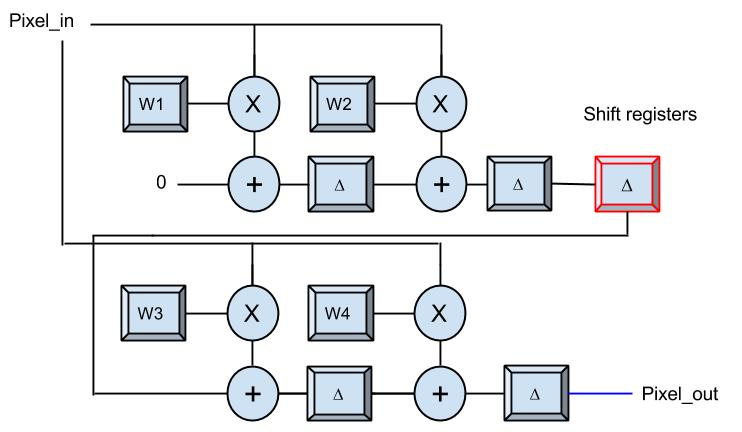
\includegraphics[width=0.7\textwidth]{Figures/Method/Convolver}
  \caption[The convoluter ]{The convoluter, when $ n = 3 $ and $ k = 2 $.}
\end{figure}
	
By providing this delay you only have to input each pixel once during the convolution. Generally every pixel is needed for $ k \times k $ convolution operations (the exception being the pixels close to the boarders of the image). Thus the shift registers are used to store the intermediate values of the convolutions until a pixel that is needed for the respective convolution operation is inputted. 

The delay these shift registers cause are the reason for the delay before valid output pixels are produced. Thus from when the convolution starts, the output will not be valid before $ k-1 $ rows of the image have been processed. And for every new image row, there will be a $ k $ cycle delay before the output is valid. The reason for this delay can be intuitively understood by remembering that the input image is a $ n \times n $ matrix, while the output matrix is a $ (n-k+1) \times (n-k+1) $ matrix. 

Since the two layers in the network have different image sizes, but use the same kernel size, we can use the module for both layers. This is done by having the control signal \textit{layer\_nr} decide how many of the shift registers that are to be used during convolution. In the first layer all of the shift registers are used, but in the second only a subset is used. I.e. $ n-k+1 $ of shift registers are used in each row, where $ n $ is either 32 or 14. 

The loading of the weights takes $ k \times k $ clock cycles, and the processing of the image takes $ n \times n $ clock cycles. Thus the total number of cycles it takes to perform a full convolution of an image is $ n \times n + k \times k $. But based upon the papers refered to in Section \ref{chap_related_work} it seems that \textit{n} tends to be larger than \textit{k}. E.g. for the first layer in the LeNet-5 \cite{LeCun1998}, $ n = 32 $ and $ k = 5 $, the loading  of the weights take 25 clock cycles and the image processing 1024 cycles. This means that the execution time of the convoluter is primairly bounded by the size of the image. But the size of the kernel decides the hardware resource cost of the module, since it requires $ k \times k $ DSP slices on the FPGA.

\begin{figure}[h!]
  \centering
      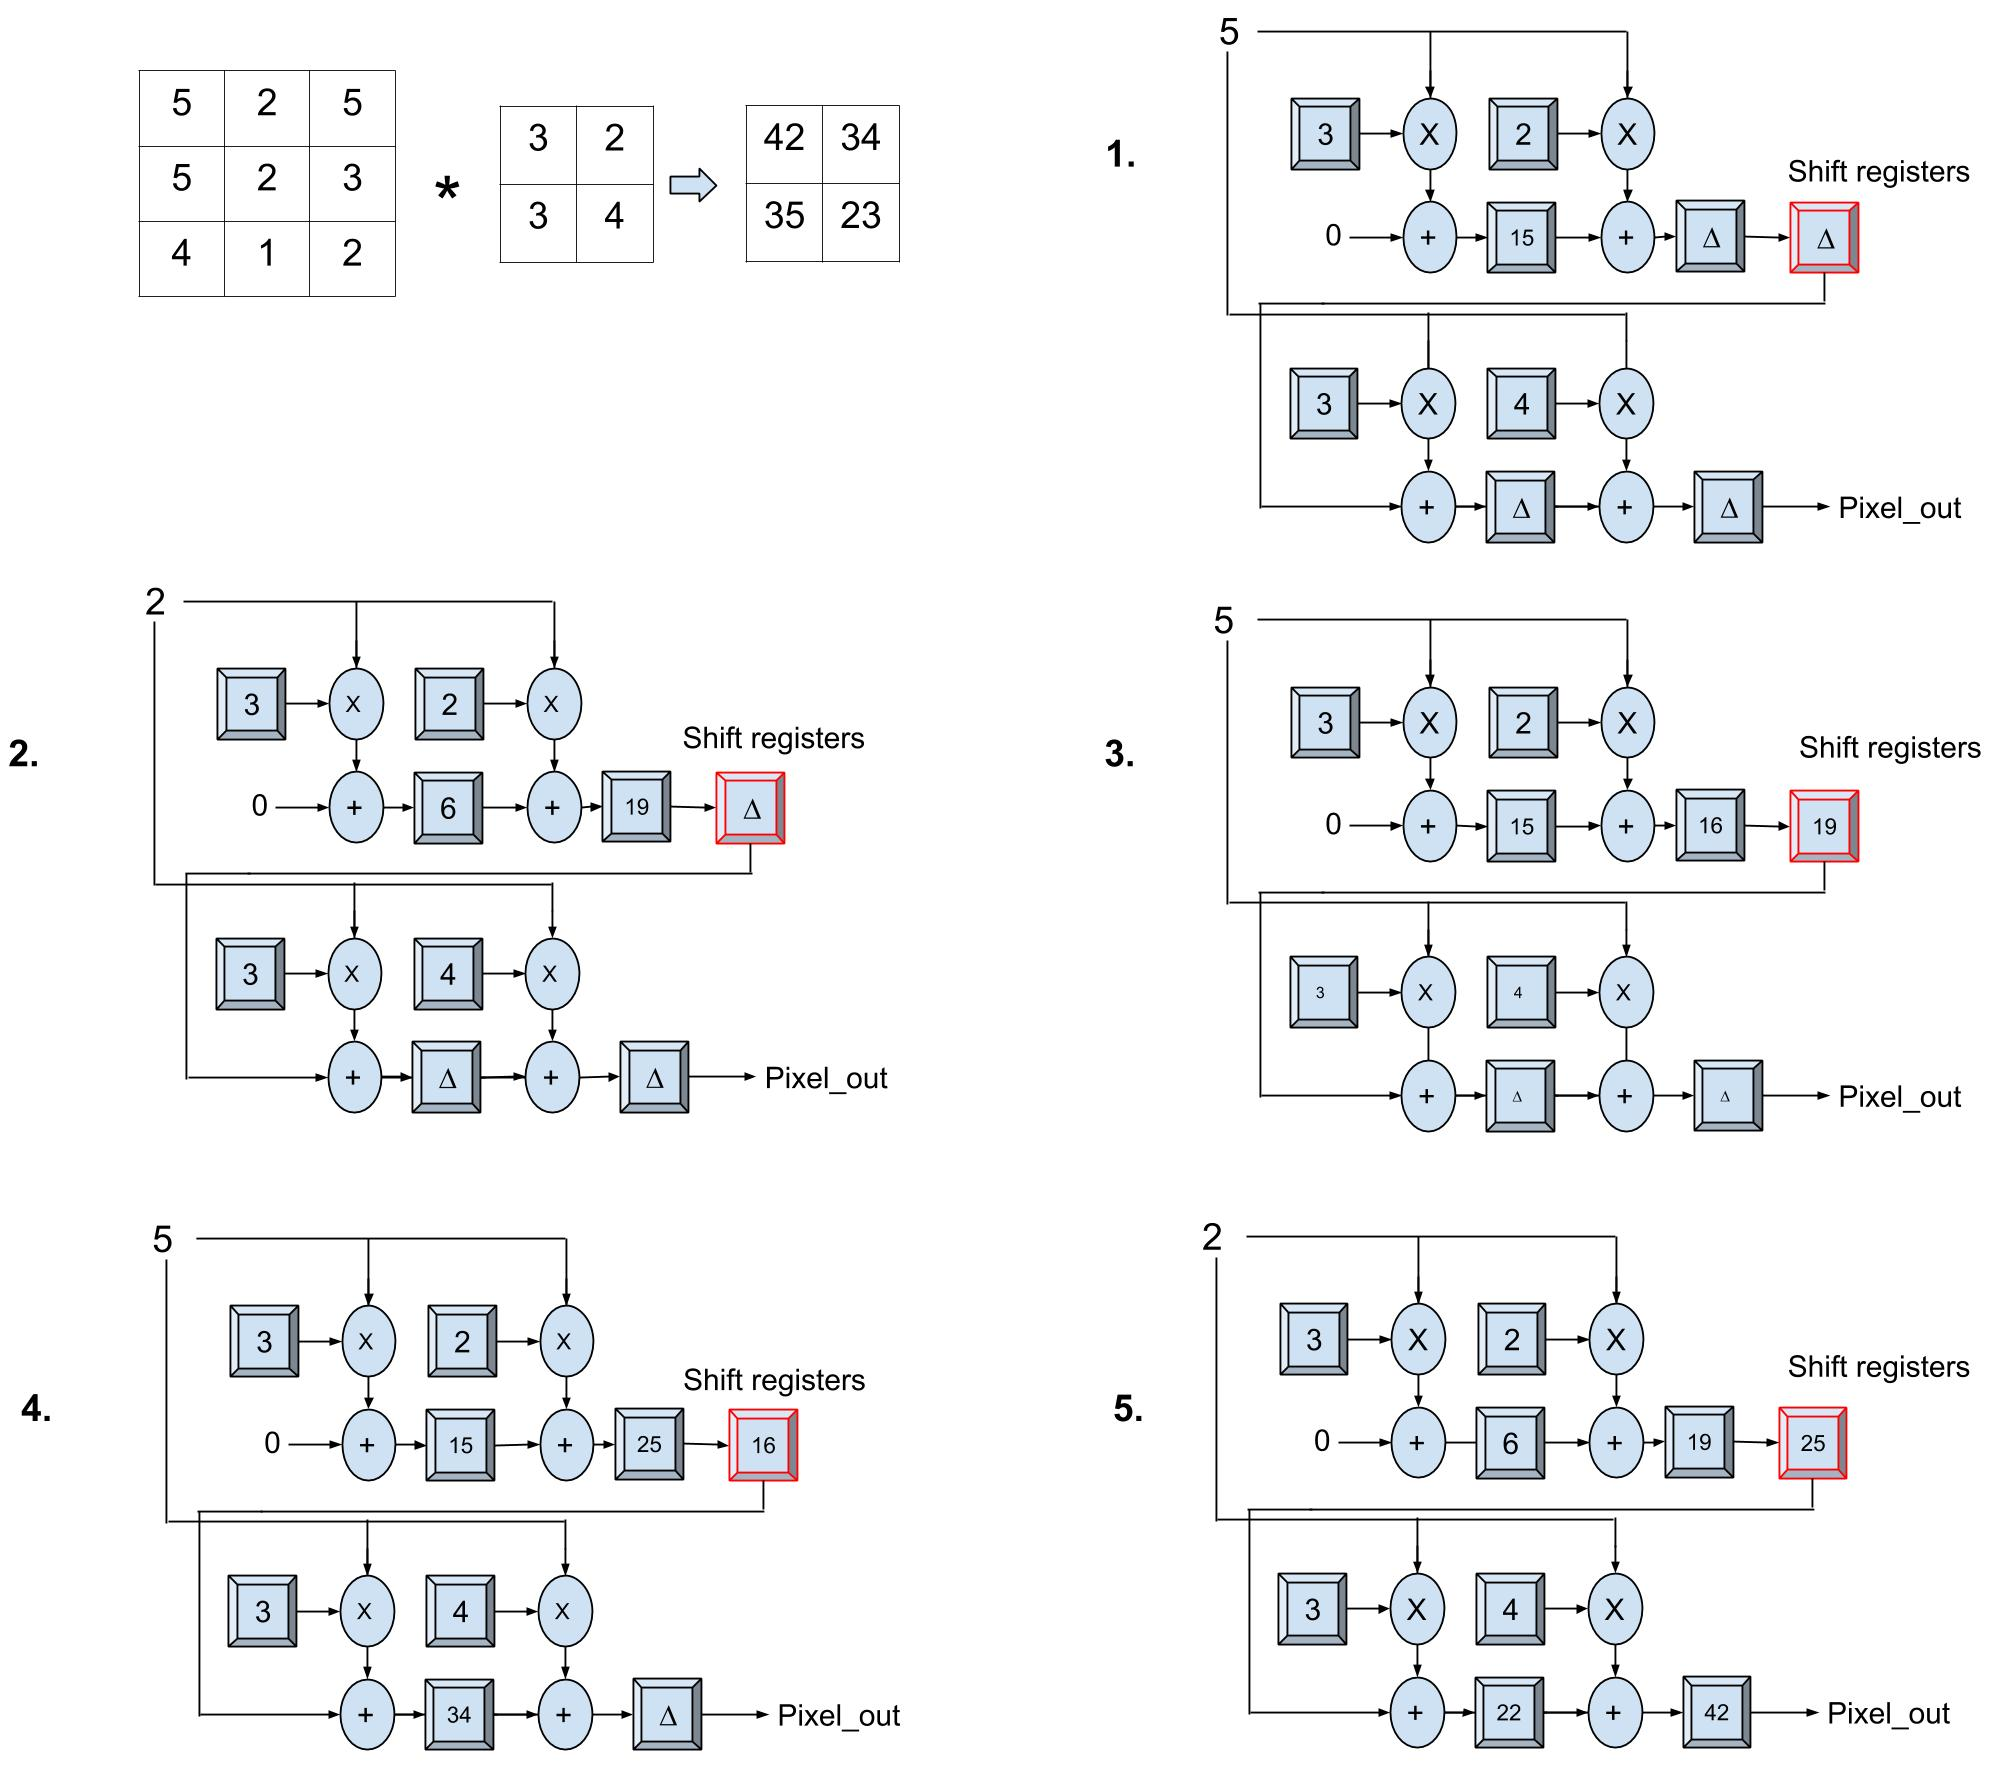
\includegraphics[width=1.1\textwidth]{Figures/Method/Conv_example}
  \caption[Convolution example]{Example showing the five first clock cycle of an convolution. The weights of the kernel is already loaded into the MAC units, and every cycle a new pixel from the image in inputted. In the last example you can see that 42 is provided as the first output.}
\end{figure}

%%%%%%%%%%%%%%%%%%%%
% HYPERBOLIC TANGENT
%%%%%%%%%%%%%%%%%%%%

\subsection{The Hyperbolic Tangent} 

This module is based upon \cite{Lin2008} using \textit{piecewise linear approximation}. It takes  as input a single value \textit{x} and outputs a linear approximation of the hyperbolic function. Using a lookup table (Table \ref{tab_tanh}) and the constants from Table \ref{tab_tanh_constants} the module decides which linear approximation to use. 
In order to meet the timing constraints on the FPGA the module has a pipeline length of three. 

\begin{table}
	\centering
    \begin{tabular}{| >{\centering\arraybackslash}m{1.2in} |} 
    \hline
    Constants \\ \hline
    $ m_1 = -0.54324 $ \\ \hline
    $ m_2 = -0.16957 $ \\ \hline
    $ c_1 = 1 $ \\ \hline
    $ c_2 = 0.42654 $ \\ \hline
    $ d_1 = 0.016 $ \\ \hline
    $ d_2 = 0.4519 $ \\ \hline
    $ a = 1.52 $ \\ \hline
    $ b = 2.57 $ \\ \hline
        \end{tabular}
    \caption{The constant used for the hyperbolic tangent approximation.}
   	\label{tab_tanh_constants}
    
    
	\centering
    \begin{tabular}{| >{\centering\arraybackslash}m{1.2in} | >{\centering\arraybackslash}m{2.5in} |} 
    \hline
    Conditions & Output \\ \hline
    $ 0 \le |x| \le a $ & $ sign(x) \times [0.5 \times m_1 \times |x|^2 + c_1 \ times |x| + d_1] $\\ \hline
    $ a \le |x| \le b $ & $ sign(x) \times [0.5 \times m_2 \times |x|^2 + c_2 \ times |x| + d_2] $\\ \hline
   	$ otherswise $ & $ signed(x) $\\ \hline
        \end{tabular}
    \caption{The piecewise linear approximation of the hyperbolic tangent.}
   	\label{tab_tanh}
    
\end{table}

\vspace*{1\baselineskip}

%%%%%%%%%%%%%%%%%%%%%%%%%%%%%%
% Average pooler
%%%%%%%%%%%%%%%%%%%%%%%%%%%%%%

\subsection{The Average Pooler} \label{sec_average_pooler}

The average pooler performs the subsample/average-pooling operation described in Section \ref{sec_cnn_def}. The input is a $ (n-k+1) \times (n-k+1) $ feature map, and the output is a $ (n-k+1)/p \times (n-k+1)/p $ subsampled/average-pooled feature map, where \textit{p} is the dimension of subsample neighborhood. 

The average pooler performs basically two operations, pooling and averaging. The input is divided into $ p \times p $ non-overlapping neighbourhoods, which are also refered to as pools. The pooling operation consist of simply summing the data within the respective neighbourhoods. The averaging operation is to multiply the summed pools with a trained average value, which produces a valid output. Figure \ref{fig_average_pooler} gives an overview of the average pooler architecture, where the SUM module and the shift registers are used for the pooling operation, while the trained C value is used to average the sums. 

Since the input is a 2D matrice that is inputted one value at a time left to right, one row at a time, the average pooler will have to keep track of data from $(n-k+1)/p $ different neighbourhoods simultaniously. That is, after the average pooler has received $ p $ inputs from the first neighbourhood, it will next receive $ p $ inputs from the next neighbourhood, and so on until the end of the first row is reached. It will then receive data from the first neighbourhood again. This will continue until it has processed $ p $ rows, after which it will have processed the first $ (n-k+1)/p $ neighbourhoods, i.e. a row of neighbourhoods. It can then continue with the next row of neighbourhoods.

In order to keep track of $ (n-k+1)/p $ neighbourhoods at a time, the average pooler contains a set of $ (n-k+1)/p - 1 $ shift registers which are used to store the intermediate sum of the neighbourhoods. The sum module keeps track of the current neighbourhood and accumulate the input data if it belongs to said neghbourhood. When a new neighbourhood is about to be inputted all the shift registers are shifted one to the right, and the sum module extracts the value of the rightmost register. 

The control unit keeps track of when to shift the registers and when a neighbourhood is fully summed. To do this the unit contains two counters, \textit{row\_num} and \textit{column\_num}. When a new pixel is inputted the \textit{column\_num} counter is incremented, and when it reaches the end of the row the \textit{row\_num} counter is incremented. Every time $ column\_num~mod~p = 0 $ another pool is encounted, and the shift registers are shifted one to the right. When $ column\_num~mod~p = 0 $ and $ row\_num~mod~p = 0 $ the final value in a pool has been reached, and the final sum is multiplied with the trained value C and outputted. 

\begin{figure}[h!]
  \centering
      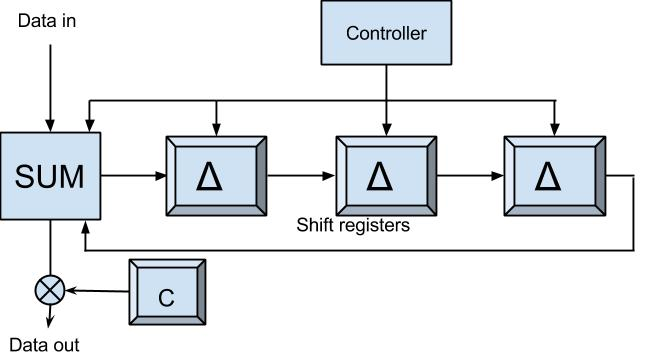
\includegraphics[width=0.5\textwidth]{Figures/Method/submax}
  \caption{The average pooler. The summation module and the shift registers are used to sum up the respective pools. The trained value C is used to average the summed pools.}
  \label{fig_average_pooler}
\end{figure}

The execution speed of the average pooler module is bounded by the size of the feature map, $ (n-k+1) \times (n-k+1) $ clock cycles, finishing one cycle after the last pixel has been inputted. Thus by streaming the output of the convoluter to the average pooler, both will finish only a few cycles apart, effectively running both jobs in parallel. The resource usage of the module is bounded by the size of the subsampling dimension, since it requires a number of shift registers equal to the size of the dimension. In addition is consumes one DSP, which is used for the averaging operation at the end. But essentially its resource usage is quite low.  

